% Options for packages loaded elsewhere
\PassOptionsToPackage{unicode}{hyperref}
\PassOptionsToPackage{hyphens}{url}
\PassOptionsToPackage{dvipsnames,svgnames,x11names}{xcolor}
\documentclass[
  10pt,
]{article}
\usepackage{xcolor}
\usepackage[margin=1in]{geometry}
\usepackage{amsmath,amssymb}
\setcounter{secnumdepth}{-\maxdimen} % remove section numbering
\usepackage{iftex}
\ifPDFTeX
  \usepackage[T1]{fontenc}
  \usepackage[utf8]{inputenc}
  \usepackage{textcomp} % provide euro and other symbols
\else % if luatex or xetex
  \usepackage{unicode-math} % this also loads fontspec
  \defaultfontfeatures{Scale=MatchLowercase}
  \defaultfontfeatures[\rmfamily]{Ligatures=TeX,Scale=1}
\fi
\usepackage{lmodern}
\ifPDFTeX\else
  % xetex/luatex font selection
\fi
% Use upquote if available, for straight quotes in verbatim environments
\IfFileExists{upquote.sty}{\usepackage{upquote}}{}
\IfFileExists{microtype.sty}{% use microtype if available
  \usepackage[]{microtype}
  \UseMicrotypeSet[protrusion]{basicmath} % disable protrusion for tt fonts
}{}
\makeatletter
\@ifundefined{KOMAClassName}{% if non-KOMA class
  \IfFileExists{parskip.sty}{%
    \usepackage{parskip}
  }{% else
    \setlength{\parindent}{0pt}
    \setlength{\parskip}{6pt plus 2pt minus 1pt}}
}{% if KOMA class
  \KOMAoptions{parskip=half}}
\makeatother
\usepackage{longtable,booktabs,array}
\newcounter{none} % for unnumbered tables
\usepackage{calc} % for calculating minipage widths
% Correct order of tables after \paragraph or \subparagraph
\usepackage{etoolbox}
\makeatletter
\patchcmd\longtable{\par}{\if@noskipsec\mbox{}\fi\par}{}{}
\makeatother
% Allow footnotes in longtable head/foot
\IfFileExists{footnotehyper.sty}{\usepackage{footnotehyper}}{\usepackage{footnote}}
\makesavenoteenv{longtable}
\usepackage{graphicx}
\makeatletter
\newsavebox\pandoc@box
\newcommand*\pandocbounded[1]{% scales image to fit in text height/width
  \sbox\pandoc@box{#1}%
  \Gscale@div\@tempa{\textheight}{\dimexpr\ht\pandoc@box+\dp\pandoc@box\relax}%
  \Gscale@div\@tempb{\linewidth}{\wd\pandoc@box}%
  \ifdim\@tempb\p@<\@tempa\p@\let\@tempa\@tempb\fi% select the smaller of both
  \ifdim\@tempa\p@<\p@\scalebox{\@tempa}{\usebox\pandoc@box}%
  \else\usebox{\pandoc@box}%
  \fi%
}
% Set default figure placement to htbp
\def\fps@figure{htbp}
\makeatother
\setlength{\emergencystretch}{3em} % prevent overfull lines
\providecommand{\tightlist}{%
  \setlength{\itemsep}{0pt}\setlength{\parskip}{0pt}}

\usepackage{newunicodechar}
\newunicodechar{τ}{\ensuremath{\tau}}\newunicodechar{ε}{\ensuremath{\varepsilon}}\newunicodechar{λ}{\ensuremath{\lambda}}
\newunicodechar{μ}{\ensuremath{\mu}}\newunicodechar{α}{\ensuremath{\alpha}}\newunicodechar{ρ}{\ensuremath{\rho}}
\newunicodechar{π}{\ensuremath{\pi}}\newunicodechar{η}{\ensuremath{\eta}}\newunicodechar{δ}{\ensuremath{\delta}}
\newunicodechar{∈}{\ensuremath{\in}}\newunicodechar{≥}{\ensuremath{\geq}}\newunicodechar{≤}{\ensuremath{\leq}}
\newunicodechar{−}{\ensuremath{-}}\newunicodechar{×}{\ensuremath{\times}}\newunicodechar{±}{\ensuremath{\pm}}
\newunicodechar{·}{\ensuremath{\cdot}}\newunicodechar{√}{\ensuremath{\surd}}\newunicodechar{…}{\ldots}
\usepackage{fancyvrb}
\RecustomVerbatimEnvironment{verbatim}{Verbatim}{fontsize=\scriptsize}
\usepackage{float}
\usepackage{etoolbox}
\AtBeginEnvironment{longtable}{\small}
\setlength{\emergencystretch}{3em}
\usepackage{bookmark}
\IfFileExists{xurl.sty}{\usepackage{xurl}}{} % add URL line breaks if available
\urlstyle{same}
\hypersetup{
  pdftitle={FRUGAL-AI: A Cost-Aware Adaptive Framework for Reducing LLM Inference Cost},
  pdfauthor={Vijayakumar Gurusamy Raju Independent Researcher},
  colorlinks=true,
  linkcolor={black},
  filecolor={Maroon},
  citecolor={Blue},
  urlcolor={blue},
  pdfcreator={LaTeX via pandoc}}

\title{FRUGAL-AI: A Cost-Aware Adaptive Framework for Reducing LLM
Inference Cost}
\author{Vijayakumar Gurusamy Raju\\ Independent Researcher}
\date{}

\begin{document}
\maketitle
\begin{abstract}
Large language model (LLM) inference now dominates the operating cost of
AI applications, yet most production systems send every request to a
single large model regardless of difficulty. Caching, routing and
cascading each cut this cost, but they are usually studied one at a time
and tuned to a quality target that is then missed on new data. We
present FRUGAL-AI, a model-agnostic serving pipeline that combines a
semantic cache, a difficulty router and a verifier-gated cascade, and
calibrates all of their thresholds jointly against one quality target
with a statistical margin. An online multiplier holds spend to a budget
when traffic shifts. We evaluate on 885 queries from five benchmarks
(multiple-choice question answering, competition mathematics,
competitive programming, summarization and multi-turn dialogue) with a
three-model Claude pool. At a target of 98\% of the largest model's
quality, on a stream with 30\% repeated requests, FRUGAL-AI cuts cost by
50.8\% (± 5.2) and retains 98.5\% of quality, against 20.5\% for routing
alone and 25.9\% for caching alone. At matched quality on distinct
queries it saves 21 points more than routing alone at 98\% quality
retained (p = 0.003) and 12 points more at 98.5\% (p = 0.04); at 99\%
the two are statistically tied. We also report what did not work: prompt
compression was never worth its quality loss, an online quality
controller fed by a 2\% audit sample gave no gain over the calibrated
settings, a cascade without a router saved almost nothing, and
per-workload quality floors could not be calibrated reliably for the
full pipeline from 40 to 200 queries per workload. The online budget
multiplier cut the share of windows over budget after a traffic shift
from 86\% to 9\%, at a cost of about 4 points of quality. The code, the
logged model outputs and the evaluation protocol are available at
https://github.com/vijayakumargr/frugal-ai.

\textbf{Keywords:} large language models; inference cost optimization;
model routing; model cascades; semantic caching; prompt compression;
constrained optimization; green AI
\end{abstract}

\subsection{1. Introduction}\label{introduction}

Most LLM spend is wasted on queries that a smaller model, a cached
answer or a shorter prompt could serve equally well. Commercial APIs
price per token, and the price gap between small and frontier models is
often one to two orders of magnitude. Self-hosted deployments face the
same gap in GPU hours and energy.

In practice, query difficulty is highly skewed. A large share of traffic
in assistants, support bots and retrieval-augmented generation (RAG)
systems is routine: greetings, FAQs, lookups and reformatting. Only a
minority of requests needs multi-step reasoning. Sending all requests to
the strongest model buys quality that most queries do not need.

Prior work mostly attacks this waste one technique at a time: caching,
routing, cascading or prompt compression. Recent work adds online budget
control to routing and statistical guarantees to cascades, but each
still tunes one component. Two practical questions remain open. First,
how much do the techniques add to each other when they are tuned
together against a single quality target? Second, does a system tuned to
a target on calibration data actually meet it on new traffic? Reported
savings are hard to compare when methods land at different quality
levels.

\textbf{Research questions.}

\begin{enumerate}
\def\labelenumi{\arabic{enumi}.}
\tightlist
\item
  RQ1: How much cost can a combined pipeline save, at a fixed quality
  target, compared with each technique alone?
\item
  RQ2: Can an online controller keep quality above a target and spend
  under a budget as traffic shifts?
\item
  RQ3: Which components contribute most, and do their gains add up or
  overlap?
\end{enumerate}

\textbf{Contributions.}

\begin{itemize}
\tightlist
\item
  A serving pipeline, FRUGAL-AI, that composes a semantic cache, a
  difficulty router and a verifier-gated cascade, with all thresholds
  calibrated jointly against one quality target, a margin for sampling
  error and a share of the tolerance reserved for wrong cache hits.
\item
  A formulation of LLM serving as constrained expected-cost
  minimization, with a primal-dual controller whose budget multiplier we
  show to hold spend under a traffic shift.
\item
  A controlled evaluation on logged outputs of three models, in which
  every method is scored on identical answers and compared both at a
  common target and at matched achieved quality.
\item
  Negative results reported in full: prompt compression, an audit-driven
  online quality controller and per-workload quality floors did not pay
  off in this setting, and a cascade without a router saved almost
  nothing.
\item
  An open-source implementation and the logged model outputs, so that
  all tables can be reproduced without new model calls.
\end{itemize}

Section 2 reviews related work. Section 3 states the problem, Section 4
describes the framework and Section 5 its algorithms. Sections 6 and 7
present the experiments, and Sections 8 and 9 discuss limitations and
conclude.

\subsection{2. Related Work}\label{related-work}

Existing cost-reduction methods each tune one source of waste. FRUGAL-AI
calibrates the cache, router and cascade together, and our contribution
is the measurement of what that joint calibration gains and where it
fails, not a claim to the first budget-controlled router.

\textbf{Model cascades and routing.} FrugalGPT {[}1{]} showed that a
cascade of LLM APIs with a learned scorer can match a strong model at
lower cost. Hybrid LLM {[}2{]} and RouteLLM {[}3{]} train routers that
choose between a small and a large model per query, using preference
data. AutoMix {[}4{]} lets a small model self-verify and escalate. These
methods use fixed thresholds and do not adapt to budget or traffic
drift.

Online and guaranteed routing (2025--2026). Several recent works close
the gap on adaptation; a survey is given in {[}37{]}. ParetoBandit
{[}30{]} and WISERouter {[}31{]} treat routing as a constrained
contextual bandit with online budget pacing, GAR {[}32{]} uses an online
primal-dual router with accuracy floors, and Panda et al.~{[}33{]} give
a bandit router under a budget. Cascade routing {[}34{]} unifies routing
and cascading in one decision rule. Conformal Cascade {[}35{]} and C3PO
{[}36{]} give distribution-free guarantees for cascade deferral and
cascade cost. These works control one component, the router or the
cascade; none calibrates a semantic cache together with them, and none
reports whether the calibrated quality target is met on held-out traffic
for a full pipeline. We did not implement them as baselines (Section 8).

\textbf{Caching.} GPTCache {[}5{]} reuses answers for semantically
similar queries using embedding search. Key-value cache reuse and paged
attention {[}6{]} reduce serving cost inside the model server but do not
avoid model calls.

\textbf{Prompt compression.} Selective Context {[}7{]} and LLMLingua
{[}8{]}, {[}9{]} drop low-information tokens using a small language
model, reducing input tokens with modest quality loss.

\textbf{Model compression and efficient decoding.} Distillation
{[}10{]}, quantization such as GPTQ {[}11{]} and AWQ {[}12{]}, and
speculative decoding {[}13{]} make each call cheaper. They are
orthogonal to FRUGAL-AI and can be applied to any model in its pool.

\textbf{Constrained online learning.} Bandits with knapsacks {[}14{]}
and online convex optimization with long-term constraints {[}15{]},
{[}16{]} give the tools we use to keep spend and quality within limits
over time.

\textbf{Green AI.} Strubell et al.~{[}17{]} and Schwartz et al.~{[}18{]}
argue for reporting compute and energy cost alongside accuracy, which
motivates our evaluation protocol.

{\def\LTcaptype{none} % do not increment counter
\begin{longtable}[]{@{}
  >{\raggedright\arraybackslash}p{(\linewidth - 12\tabcolsep) * \real{0.2154}}
  >{\raggedright\arraybackslash}p{(\linewidth - 12\tabcolsep) * \real{0.0846}}
  >{\raggedright\arraybackslash}p{(\linewidth - 12\tabcolsep) * \real{0.1231}}
  >{\raggedright\arraybackslash}p{(\linewidth - 12\tabcolsep) * \real{0.1154}}
  >{\raggedright\arraybackslash}p{(\linewidth - 12\tabcolsep) * \real{0.0846}}
  >{\raggedright\arraybackslash}p{(\linewidth - 12\tabcolsep) * \real{0.1615}}
  >{\raggedright\arraybackslash}p{(\linewidth - 12\tabcolsep) * \real{0.2154}}@{}}
\toprule\noalign{}
\begin{minipage}[b]{\linewidth}\raggedright
Approach
\end{minipage} & \begin{minipage}[b]{\linewidth}\raggedright
Cache
\end{minipage} & \begin{minipage}[b]{\linewidth}\raggedright
Compress prompt
\end{minipage} & \begin{minipage}[b]{\linewidth}\raggedright
Route per query
\end{minipage} & \begin{minipage}[b]{\linewidth}\raggedright
Cascade
\end{minipage} & \begin{minipage}[b]{\linewidth}\raggedright
Budget control online
\end{minipage} & \begin{minipage}[b]{\linewidth}\raggedright
Quality target calibrated
\end{minipage} \\
\midrule\noalign{}
\endhead
\bottomrule\noalign{}
\endlastfoot
FrugalGPT {[}1{]} & yes & partial & no & yes & no & no \\
Hybrid LLM {[}2{]} & no & no & yes & no & no & no \\
RouteLLM {[}3{]} & no & no & yes & no & no & no \\
AutoMix {[}4{]} & no & no & no & yes & no & no \\
GPTCache {[}5{]} & yes & no & no & no & no & no \\
LLMLingua {[}8{]} & no & yes & no & no & no & no \\
ParetoBandit {[}30{]}, WISERouter {[}31{]} & no & no & yes & no & yes &
no \\
Cascade routing {[}34{]} & no & no & yes & yes & no & no \\
Conformal Cascade {[}35{]} & no & no & no & yes & no & yes, for the
cascade \\
FRUGAL-AI (ours) & yes & optional, unused & yes & yes & yes & yes,
jointly, with a margin; met in 70\% of seeds \\
\end{longtable}
}

\subsection{3. Problem Formulation}\label{problem-formulation}

We cast LLM serving as choosing, per query, the cheapest action whose
expected quality keeps the long-run average above a target.

Let M = \{\(m_1\), \ldots, \(m_K\)\} be a pool of models ordered by
per-token price. For a query x, model \(m_k\) incurs cost \(c_k(x)\) =
\(p_k^{\mathrm{in}}\) · \(n_{\mathrm{in}}(x)\) + \(p_k^{\mathrm{out}}\)
· \(n_{\mathrm{out}}(x)\), where \(p_k\) are the input and output prices
per token and n are token counts. A quality function Q(y, x) ∈ {[}0,
1{]} scores the answer y, using task metrics or an LLM judge.

A serving policy π maps each query to an action a ∈ A: return a cached
answer, compress the prompt, call one model, or run a cascade of models.
Let \(C_\pi(x)\) and \(Q_\pi(x)\) be the realized cost and quality.
Given a quality target \(q^{*}\) and a per-request budget B, we solve:

\[
\min_{\pi} \; \mathbb{E}_{x \sim \mathcal{D}}\big[C_\pi(x)\big]
\quad \text{s.t.} \quad
\mathbb{E}_{x \sim \mathcal{D}}\big[Q_\pi(x)\big] \ge q^{*},
\qquad
\mathbb{E}_{x \sim \mathcal{D}}\big[C_\pi(x)\big] \le B
\]

In practice \(q^{*}\) is set relative to a reference policy that always
calls the strongest model \(m_K\), for example \(q^{*}\) = (1 − ε) ·
\(\mathbb{E}[Q_K(x)]\) with tolerance ε such as 0.01 or 0.02.

The Lagrangian relaxation with multiplier λ ≥ 0 gives a per-query rule:
choose the action that minimizes predicted cost minus λ times predicted
quality.

\[
a^{*}(x) = \arg\min_{a \in \mathcal{A}} \; \hat{c}_a(x) - \lambda \, \hat{q}_a(x)
\]

Here \(\hat{c}\) and \(\hat{q}\) are learned estimates. A large λ favors
quality and a small λ favors savings. Section 5 shows how λ is adjusted
online so that both constraints hold over time.

For a cascade that tries models \(k_1 < k_2 < \dots < k_J\) in order and
stops at stage j when a verifier accepts, the expected cost is:

\[
\mathbb{E}[C_{\text{cascade}}(x)] = \sum_{j=1}^{J} \big(c_{k_j}(x) + v_{k_j}(x)\big) \cdot \prod_{i<j} \big(1 - \alpha_{k_i}(x)\big)
\]

where v is the verifier cost and \(\alpha_k(x)\) is the probability that
the verifier accepts the answer of \(m_k\). Note that the product
multiplies both terms in the sum. A cascade pays off only when cheap
stages are accepted often enough to offset the cost of failed attempts.

\subsection{4. The FRUGAL-AI Framework}\label{the-frugal-ai-framework}

FRUGAL-AI is a pipeline in front of a model pool: a semantic cache, an
optional prompt compressor, a difficulty router and a verifier-gated
cascade. Each stage can end the request early, and one calibration step
sets all thresholds against a single quality target. In the
configuration evaluated as FRUGAL-AI in Section 7 the compressor is
switched off.

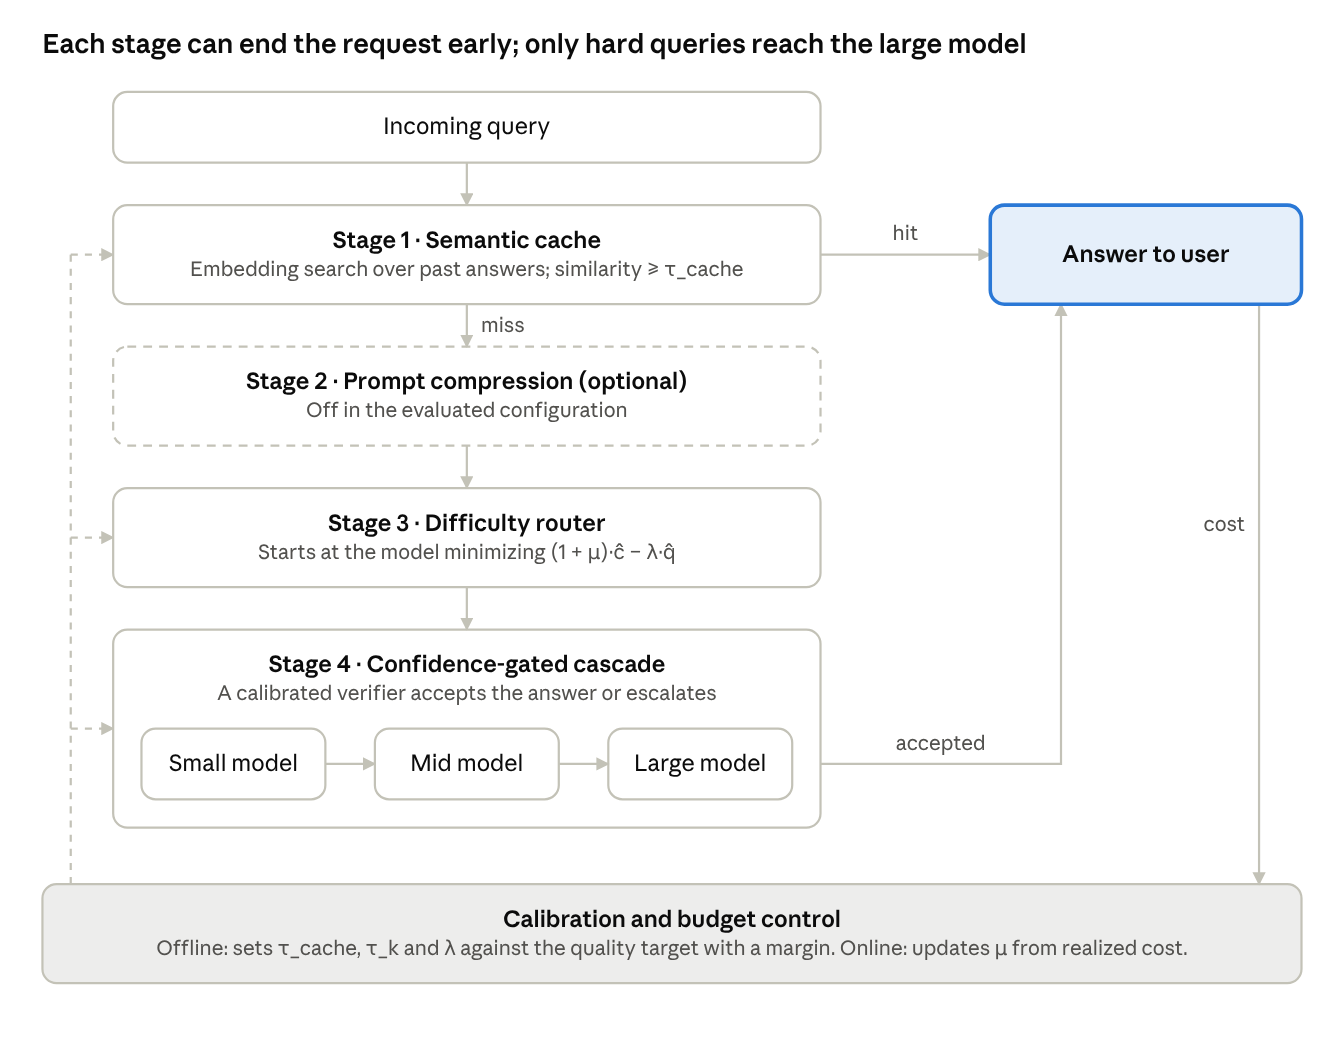
\includegraphics[width=0.92\linewidth,height=\textheight,keepaspectratio]{fig1_pipeline.png}

Figure 1. A cache hit or an accepted cascade answer ends the request.
The thresholds are calibrated offline against the quality target, and
the budget multiplier μ is updated online from realized cost. Prompt
compression (dashed) is optional and off in the evaluated configuration.

\subsubsection{4.1 Stage 1: Semantic
cache}\label{stage-1-semantic-cache}

Each query is embedded with a small sentence encoder and searched in a
vector index of past (query, answer) pairs. If the nearest neighbour has
cosine similarity above \(\tau_{\mathrm{cache}}\) and the cached answer
passed verification, it is returned at near-zero cost. To limit stale or
wrong reuse, entries carry a time-to-live, and the cache is keyed on the
query plus a hash of any retrieved context. The threshold
\(\tau_{\mathrm{cache}}\) is the lowest value whose conformal bound on
the false-hit rate, measured on a calibration replay stream, stays
within the cache's share of the quality tolerance. We reserve a quarter
of the tolerance ε for wrong cache hits, so at ε = 0.02 the bound is
0.5\%.

\subsubsection{4.2 Stage 2: Task-aware prompt
compression}\label{stage-2-task-aware-prompt-compression}

Long prompts in RAG and multi-turn chat dominate input cost. A small
model scores each context sentence for relevance to the query, using
token-level information in the style of {[}7{]}, {[}8{]}. Sentences
below a learned keep-ratio r are dropped, while instructions, the query
and code blocks are always kept. The ratio r is chosen per task to bound
the predicted quality loss.

In our implementation the compressor keeps the half of the document
sentences most similar to the query. The compressed prompt is one more
action the router may choose. On the summarization workload it lowered
the judged score from about 0.80 to about 0.70, so the calibration never
selected it at the targets we tested; the stage is therefore off by
default and reported as an ablation.

\subsubsection{4.3 Stage 3: Difficulty-aware
router}\label{stage-3-difficulty-aware-router}

The router predicts, for each model \(m_k\), the probability
\(\hat{q}_k(x)\) that \(m_k\)'s answer meets the quality bar. It is a
light classifier, such as a fine-tuned small encoder or gradient-boosted
trees on embeddings plus features like query length, domain tag and
presence of code or math. Training labels come from running all pool
models on a training set and scoring their answers. The router then
applies the Lagrangian rule from Section 3 to pick either a single model
or the starting point of a cascade.

\subsubsection{4.4 Stage 4: Confidence-gated
cascade}\label{stage-4-confidence-gated-cascade}

If the router starts at a cheaper model, a verifier decides whether to
accept its answer or escalate to the next model. The verifier is one
call to the small model that rates the answer's correctness from 0 to
100; the API exposes no token log-probabilities. A logistic model
calibrates this rating, together with the router's prior, into a
probability that the answer is good. The acceptance threshold \(\tau_k\)
is set with conformal risk control {[}26{]}, which bounds the expected
quality lost to wrongly accepted answers by a level α.

\subsubsection{4.5 Budget controller}\label{budget-controller}

Offline calibration. The controller first sets the cache threshold, the
cascade risk level α (and with it the thresholds \(\tau_k\)) and the
quality multiplier λ on the calibration split. It lists every candidate
setting with its mean cost and quality, keeps the cost-quality front,
and walks that front from the safest setting towards cheaper ones. A
setting is accepted while its mean quality exceeds the target by one
standard error of the paired difference to the reference model; the walk
stops at the first setting that fails. The routing stages are calibrated
to three quarters of the tolerance ε, and the cache to the remaining
quarter. The same rule is applied to every tuned baseline.

Online control. While serving, the controller updates the budget
multiplier μ with the primal-dual rule in Section 5; a positive μ also
lowers \(\tau_k\), so more cheap answers are accepted under budget
pressure. An online quality multiplier, driven by a random audit sample
that also calls the reference model (2\% of traffic, with the audit
calls counted in the cost), is available as an option. It gave no gain
in our experiments and is off by default.

\subsubsection{4.6 Design properties}\label{design-properties}

\begin{itemize}
\tightlist
\item
  \textbf{Model-agnostic:} works with API models and self-hosted models,
  and with compressed or quantized models in the pool.
\item
  \textbf{Composable:} each stage can be switched off, which enables the
  ablations in Section 7.
\item
  \textbf{Low overhead:} all control components are small models that
  run on CPU or a shared GPU.
\end{itemize}

\subsection{5. Algorithms}\label{algorithms}

This section gives the two multiplier updates used online, the
calibration and serving algorithms, and their relation to existing
theory. In our experiments only the budget multiplier was effective;
Section 7.2 reports why the quality multiplier was not.

\subsubsection{5.1 Online primal-dual
control}\label{online-primal-dual-control}

We keep two multipliers: \(\lambda_t\) for the quality constraint and
\(\mu_t\) for the budget constraint. At each request t the router picks
the action that minimizes the per-query Lagrangian:

\[
a_t = \arg\min_{a \in \mathcal{A}} \; (1 + \mu_t)\,\hat{c}_a(x_t) - \lambda_t\,\hat{q}_a(x_t)
\]

After serving, the controller updates the multipliers by projected
subgradient steps with step size η:

\[
\lambda_{t+1} = \big[\lambda_t + \eta\,(q^{*} - \tilde{Q}_t)\big]_{+},
\qquad
\mu_{t+1} = \big[\mu_t + \eta\,(C_t - B)\big]_{+}
\]

In the implementation, cost is measured in units of the reference
model's mean cost, and a positive μ also divides the acceptance
thresholds \(\tau_k\) by 1 + μ. Quality is observed only on audited
requests, a random share ρ of traffic on which the reference model also
answers. On those requests the quality step uses the gap between (1 − ε)
times the reference answer's quality and the served answer's quality,
scaled by 1/ρ so that the update is unbiased; on all other requests λ is
unchanged. The quality update is optional and off in the default
configuration.

\subsubsection{5.2 Algorithms 1 and 2: calibration and
serving}\label{algorithms-1-and-2-calibration-and-serving}

Algorithm 1 is run once on the calibration split and fixes the cache
threshold, the cascade thresholds and the quality multiplier. Algorithm
2 then serves requests with those settings and, when a budget is given,
updates the budget multiplier.

\begin{verbatim}
# Algorithm 1: offline calibration (calibration split only, pseudocode)
def calibrate(settings, ref_quality, eps, z=1.0, cache_share=0.25):
    # Cache: lowest threshold whose conformal bound on wrong hits fits its share.
    tau_cache = min(t for t in cache_grid
                    if (false_hits(t) + 1) / (n_requests + 1) <= cache_share * eps)
    # Routing and cascade: the rest of the tolerance, per query.
    target = (1 - (1 - cache_share) * eps) * ref_quality
    front = pareto_front(settings)        # by mean cost and mean quality
    chosen = front.safest()               # always-large
    for s in front.from_safest_to_cheapest():
        d = s.quality - target            # paired difference per query
        if mean(d) - z * stderr(d) < 0:
            break                         # the first failure ends the walk
        chosen = s
    return tau_cache, chosen.tau, chosen.lam
\end{verbatim}

\begin{verbatim}
# Algorithm 2: serving loop, default configuration (pseudocode)
mu = 0.0
for x in stream:
    hit = cache.lookup(embed(x), tau_cache)
    if hit is not None:
        y, cost = hit.answer, 0.0
    else:
        q_hat, c_hat = router.predict(x)  # expected cascade quality and cost per start model
        k = argmin((1 + mu) * c_hat - lam * q_hat)
        cost = 0.0
        while True:
            y = models[k].generate(x)
            cost += price(k, x, y)
            if k == K - 1:
                break                     # the largest model's answer is final
            cost += verifier_price
            if verifier.score(x, y) >= tau[k] / (1 + mu):
                break                     # accepted; budget pressure relaxes acceptance
            k += 1                        # escalate
        cache.insert(x, y)
    if budget is not None:
        mu = max(0.0, mu + eta_mu * (cost / ref_cost - budget))
    yield y
# Options, off by default: a compressed prompt as an extra action for the router,
# and the audit-driven update of lam from Section 5.1.
\end{verbatim}

\subsubsection{5.3 Relation to existing
theory}\label{relation-to-existing-theory}

We do not claim a new theoretical result. The multiplier updates of
Section 5.1 follow the dual-subgradient scheme analysed for online
convex optimization with long-term constraints {[}15{]} and with
stochastic constraints {[}16{]}; for i.i.d. requests and a strictly
feasible policy, the latter gives expected regret and constraint
violation of order \(\sqrt{T}\). Our setting departs from the
assumptions of those results in three ways: the action set is discrete
and chosen through learned cost and quality estimates, quality is
observed only on a small audit sample, and traffic may shift. The bounds
therefore do not transfer directly, and we make no formal claim for the
online controller. Empirically (Section 7.2) the budget multiplier held
spend under a shift, while the quality multiplier, with about 10 audit
labels per 500 requests, did not track quality.

The offline calibration gives a different kind of assurance. For each
cascade threshold taken alone, conformal risk control {[}26{]} bounds
the expected quality lost to wrongly accepted answers by α under
exchangeability, and the same conformal correction bounds the cache's
false-hit rate. The joint choice of the risk level and the multiplier in
Algorithm 1, with its one-standard-error margin and its stop at the
first failing setting, is a heuristic for which we give no guarantee.
Section 7 therefore reports how often the target is met on held-out
data.

\subsubsection{5.4 Complexity and
overhead}\label{complexity-and-overhead}

Per request, the cache lookup costs O(log N) with an approximate
nearest-neighbour index over N entries. The router and cost model cost
one small forward pass each. The cascade adds at most K − 1 extra model
calls in the worst case, and the controller update is O(1). We report
measured overhead in Section 7.

\subsection{6. Experimental Setup}\label{experimental-setup}

We evaluate on five public workloads with a three-tier model pool and
compare against six baselines at matched quality targets.

\subsubsection{6.1 Workloads}\label{workloads}

{\def\LTcaptype{none} % do not increment counter
\begin{longtable}[]{@{}
  >{\raggedright\arraybackslash}p{(\linewidth - 8\tabcolsep) * \real{0.2276}}
  >{\raggedright\arraybackslash}p{(\linewidth - 8\tabcolsep) * \real{0.0894}}
  >{\raggedright\arraybackslash}p{(\linewidth - 8\tabcolsep) * \real{0.2276}}
  >{\raggedright\arraybackslash}p{(\linewidth - 8\tabcolsep) * \real{0.2276}}
  >{\raggedright\arraybackslash}p{(\linewidth - 8\tabcolsep) * \real{0.2276}}@{}}
\toprule\noalign{}
\begin{minipage}[b]{\linewidth}\raggedright
Workload
\end{minipage} & \begin{minipage}[b]{\linewidth}\raggedright
n
\end{minipage} & \begin{minipage}[b]{\linewidth}\raggedright
Task
\end{minipage} & \begin{minipage}[b]{\linewidth}\raggedright
Quality metric
\end{minipage} & \begin{minipage}[b]{\linewidth}\raggedright
Why included
\end{minipage} \\
\midrule\noalign{}
\endhead
\bottomrule\noalign{}
\endlastfoot
MMLU-Pro {[}27{]} & 400 & Multiple-choice QA with up to ten options &
Accuracy & Separates the three models \\
Codeforces problems from CodeContests {[}28{]} & 165 & Competitive
programming in Python & All hidden tests pass (up to 15 tests, 10 s
each) & Verifiable correctness; hard for small models \\
AIME 2022--2024 {[}29{]} & 90 & Competition mathematics & Exact-match
integer answer & Multi-step reasoning \\
CNN/DailyMail {[}24{]} & 150 & Long-document summarization & LLM-judge
score (1--10, scaled to 0--1) & Long prompts test compression \\
MT-Bench {[}25{]} & 80 & Multi-turn open dialogue & LLM-judge score
(1--10, scaled to 0--1) & Open-ended, assistant-like traffic \\
\end{longtable}
}

The total is 885 queries. A 100-query pilot on MMLU {[}21{]}, GSM8K
{[}22{]} and HumanEval {[}23{]} showed that the small model reached
about 98\% of the large model's quality there, so those benchmarks were
replaced with the harder ones above. To test caching, repeated and
paraphrased requests are added to the stream (Section 6.5). The
Codeforces problems date from 2021 and earlier, so the models may have
seen them in training. A real, consented production log would strengthen
the paper considerably.

\subsubsection{6.2 Model pool}\label{model-pool}

The pool has three tiers from one model family: Claude Haiku 5.5
(small), Claude Sonnet 5.5 (mid) and Claude Opus 5.5 (large, the
reference \(m_K\)), all called through the Anthropic API at the same
effort setting. Costs use list prices as of October 2026, in US dollars
per million input / output tokens: 0.10 / 0.50, 2.00 / 10.00 and 4.00 /
20.00. A single-family pool is a limitation; an open-weight tier would
test generality.

Cost accounting. Calls were made through the Claude Code command line in
non-interactive mode, with an empty system prompt and no tools, not
through the metered API. Cost is therefore computed as logged tokens
times list prices. The command line adds about 550 input tokens to every
call; this overhead was measured once per model and subtracted. The
whole collection came to 7,885 calls and 47.45 US dollars at list
prices, with no refusals, truncated answers, timeouts or judge parse
failures.

\subsubsection{6.3 Baselines}\label{baselines}

\begin{enumerate}
\def\labelenumi{\arabic{enumi}.}
\tightlist
\item
  \textbf{Always-large:} every query goes to \(m_K\) (quality
  reference).
\item
  \textbf{Always-small:} every query goes to the cheapest model (cost
  floor).
\item
  \textbf{Cache-only:} semantic cache in front of \(m_K\), as in
  {[}5{]}.
\item
  \textbf{Compression-only:} LLMLingua-style compression {[}8{]} in
  front of \(m_K\).
\item
  \textbf{Router-only:} a RouteLLM-style binary router {[}3{]}.
\item
  \textbf{Cascade-only:} FrugalGPT/AutoMix-style cascade with fixed
  thresholds {[}1{]}, {[}4{]}.
\end{enumerate}

Router-only, cascade-only and cache-only are tuned with the same
calibration rule and margin as FRUGAL-AI. We also report two variants
that calibrate one setting per workload, so that each workload must meet
the target on its own: Router-only with per-workload floors and
FRUGAL-AI with per-workload floors. The 2026 systems discussed in
Section 2 are not implemented.

\subsubsection{6.4 Metrics}\label{metrics}

\begin{itemize}
\tightlist
\item
  \textbf{Cost:} US dollars per 1,000 requests, and cost reduction
  relative to always-large.
\item
  \textbf{Quality:} task metric, and quality retained as a percentage of
  always-large.
\item
  \textbf{Pareto frontier:} cost versus quality as \(q^{*}\) sweeps from
  0.90 to 1.00 of the reference.
\item
  \textbf{Budget adherence:} share of time windows where spend exceeded
  B, and worst overshoot.
\item
  \textbf{Latency:} 95th-percentile end-to-end latency.
\item
  \textbf{Energy (optional):} estimated kWh and CO2e for self-hosted
  models, following {[}17{]}, {[}18{]}.
\end{itemize}

Two further measures make comparisons fair. Seeds meeting target is the
share of seeds in which a method's quality on the test stream reached
\(q^{*}\). Cost reduction at matched quality reads each method's saving
at a fixed quality retained (97\%, 98\%, 98.5\% and 99\%) by
interpolating along its cost-quality front on the test split, with
always-large and always-small as end points; a point between two
settings can be realized by randomizing between them.

\subsubsection{6.5 Protocol}\label{protocol}

Routers and verifiers are trained, and all thresholds calibrated, on a
50\% split that does not overlap the test split, with 5-fold
cross-fitting. All model outputs are logged once and replayed, so every
method is scored on identical outputs. Every result is the mean over 10
seeds with 95\% confidence intervals; a seed redraws the split, the
request stream and the audit sample, not the model outputs. Significance
uses paired t-tests across seeds. The main target is \(q^{*}\) = 0.98 ×
always-large (ε = 0.02); we also report ε = 0.01.

Disclosure. A first evaluation tuned every method by taking the cheapest
setting that met the target on the calibration split, at ε = 0.01 and
with 5 seeds. FRUGAL-AI then retained 97.7\% against a 99\% target, and
no tuned method reached the target on the test split. We replaced that
rule with the margin-based calibration of Section 4.5, moved the main
target to 98\% and raised the number of seeds to 10. The rule was
therefore chosen after seeing test results from the first evaluation;
the first results are kept with the released code.

The cache is tested on a replay stream in which 30\% of requests are
repeats, half of them paraphrased by the small model. This share is an
assumption and is varied from 0\% to 50\%. To test drift (RQ2), the
share of easy queries falls from 80\% to 50\% mid-stream.

\subsection{7. Results}\label{results}

At a 98\% quality target FRUGAL-AI saves about half the cost of always
calling the large model, roughly twice the saving of routing or caching
alone at similar quality; at a 99\% target its advantage over routing
shrinks to within the noise. On all 885 queries the three models score
0.824 (small), 0.856 (mid) and 0.891 (large), at 1.53, 10.71 and 22.84
US dollars per 1,000 requests. All intervals are 95\% confidence
intervals over 10 seeds. Each test split holds about 440 queries, so
differences under about 1 point of quality are not resolved.

\subsubsection{7.1 Main results (RQ1)}\label{main-results-rq1}

Table 2. Replay stream (30\% repeated requests), target \(q^{*}\) = 0.98
× always-large. Mean over 10 seeds (± 95\% CI).

{\def\LTcaptype{none} % do not increment counter
\begin{longtable}[]{@{}
  >{\raggedright\arraybackslash}p{(\linewidth - 10\tabcolsep) * \real{0.2171}}
  >{\raggedright\arraybackslash}p{(\linewidth - 10\tabcolsep) * \real{0.1860}}
  >{\raggedright\arraybackslash}p{(\linewidth - 10\tabcolsep) * \real{0.1395}}
  >{\raggedright\arraybackslash}p{(\linewidth - 10\tabcolsep) * \real{0.1550}}
  >{\raggedright\arraybackslash}p{(\linewidth - 10\tabcolsep) * \real{0.1163}}
  >{\raggedright\arraybackslash}p{(\linewidth - 10\tabcolsep) * \real{0.1860}}@{}}
\toprule\noalign{}
\begin{minipage}[b]{\linewidth}\raggedright
Method
\end{minipage} & \begin{minipage}[b]{\linewidth}\raggedright
Cost (USD / 1k requests)
\end{minipage} & \begin{minipage}[b]{\linewidth}\raggedright
Cost reduction (\%)
\end{minipage} & \begin{minipage}[b]{\linewidth}\raggedright
Quality retained (\%)
\end{minipage} & \begin{minipage}[b]{\linewidth}\raggedright
p95 latency (s)
\end{minipage} & \begin{minipage}[b]{\linewidth}\raggedright
Seeds meeting target (\%)
\end{minipage} \\
\midrule\noalign{}
\endhead
\bottomrule\noalign{}
\endlastfoot
Always-large & 22.81~±~1.84 & 0 & 100 & 40.6~±~3.0 & 100 \\
Always-small & 1.52~±~0.13 & 93.3~±~0.5 & 92.4~±~1.6 & 52.3~±~7.3 & 0 \\
Cache-only & 16.88~±~1.29 & 25.9~±~2.8 & 99.3~±~0.4 & 34.1~±~3.1 &
100 \\
Compression-only & 22.35~±~1.88 & 2.1~±~0.4 & 97.6~±~0.4 & 40.6~±~3.0 &
40 \\
Router-only & 18.19~±~2.17 & 20.5~±~4.4 & 98.7~±~1.2 & 37.3~±~3.5 &
80 \\
Cascade-only & 21.41~±~3.29 & 6.9~±~9.8 & 98.2~±~0.9 & 134.8~±~17.7 &
60 \\
FRUGAL-AI & 11.20~±~1.48 & 50.8~±~5.2 & 98.5~±~0.7 & 57.6~±~12.7 & 70 \\
Router-only, per-workload floors & 18.59~±~2.67 & 19.0~±~7.5 &
99.4~±~0.5 & 38.5~±~5.1 & 100 \\
FRUGAL-AI, per-workload floors & 13.15~±~1.57 & 42.2~±~5.8 & 97.7~±~0.8
& 65.6~±~10.3 & 30 \\
\end{longtable}
}

FRUGAL-AI costs 5.67 US dollars per 1,000 requests less than cache-only,
6.99 less than router-only and 10.20 less than cascade-only (paired
t-tests across seeds, p ≤ 0.0001 each). Its mean quality retained,
98.5\%, is above the target and within 0.2 points of router-only, but it
meets the target in 7 of 10 seeds against 8 of 10 for router-only. The
price is latency: verifier calls and escalations raise p95 latency from
40.6 s to 57.6 s. Cascade-only saves little and more than triples p95
latency, because every answer from a cheaper model also pays for a
verifier call.

Table 3. Distinct queries only (no repeats, so the cache can only do
harm), target 98\%.

{\def\LTcaptype{none} % do not increment counter
\begin{longtable}[]{@{}
  >{\raggedright\arraybackslash}p{(\linewidth - 8\tabcolsep) * \real{0.2667}}
  >{\raggedright\arraybackslash}p{(\linewidth - 8\tabcolsep) * \real{0.1714}}
  >{\raggedright\arraybackslash}p{(\linewidth - 8\tabcolsep) * \real{0.1905}}
  >{\raggedright\arraybackslash}p{(\linewidth - 8\tabcolsep) * \real{0.1429}}
  >{\raggedright\arraybackslash}p{(\linewidth - 8\tabcolsep) * \real{0.2286}}@{}}
\toprule\noalign{}
\begin{minipage}[b]{\linewidth}\raggedright
Method
\end{minipage} & \begin{minipage}[b]{\linewidth}\raggedright
Cost reduction (\%)
\end{minipage} & \begin{minipage}[b]{\linewidth}\raggedright
Quality retained (\%)
\end{minipage} & \begin{minipage}[b]{\linewidth}\raggedright
p95 latency (s)
\end{minipage} & \begin{minipage}[b]{\linewidth}\raggedright
Seeds meeting target (\%)
\end{minipage} \\
\midrule\noalign{}
\endhead
\bottomrule\noalign{}
\endlastfoot
Cache-only & 0.9~±~0.7 & 99.3~±~0.5 & 42.5~±~4.6 & 90 \\
Router-only & 21.1~±~4.8 & 98.9~±~0.6 & 40.1~±~4.4 & 90 \\
Cascade-only & 6.7~±~8.9 & 98.0~±~0.5 & 142.6~±~15.2 & 50 \\
FRUGAL-AI & 33.8~±~7.0 & 98.1~±~0.5 & 86.7~±~21.1 & 50 \\
Router-only, per-workload floors & 18.9~±~6.9 & 99.1~±~0.4 & 41.5~±~5.4
& 100 \\
FRUGAL-AI, per-workload floors & 22.8~±~7.1 & 97.6~±~0.6 & 91.1~±~17.3 &
50 \\
\end{longtable}
}

Without repeats FRUGAL-AI still saves 12.7 points more than router-only,
but it sits 0.8 points lower in quality and meets the target in only
half the seeds, so this comparison is not at equal quality. Table 5 and
Figure 2 make the comparison at matched quality.

Table 4. Stricter target, \(q^{*}\) = 0.99 × always-large. Each cell is
cost reduction (\%) / quality retained (\%) / seeds meeting target (\%).

{\def\LTcaptype{none} % do not increment counter
\begin{longtable}[]{@{}lll@{}}
\toprule\noalign{}
Method & Replay stream & Distinct queries \\
\midrule\noalign{}
\endhead
\bottomrule\noalign{}
\endlastfoot
Cache-only & 22.0~±~3.1 / 99.8 / 100 & 0.2~±~0.3 / 99.8 / 90 \\
Router-only & 15.3~±~4.2 / 99.6 / 90 & 15.5~±~3.8 / 99.4 / 90 \\
Cascade-only & −22.0~±~10.1 / 99.3 / 80 & −21.8~±~10.2 / 99.1 / 60 \\
FRUGAL-AI & 35.4~±~5.9 / 99.1 / 50 & 17.1~±~6.6 / 98.9 / 40 \\
\end{longtable}
}

At the 99\% target FRUGAL-AI's saving on the replay stream comes mostly
from the cache: on distinct queries it saves about the same as
router-only and meets the target less often. With about 440 calibration
queries, a 1\% tolerance is close to the sampling error of the quality
estimate itself, and the simpler method, with one threshold to
calibrate, is the more reliable one.

Table 5. Cost reduction (\%) at matched quality retained, distinct
queries.

{\def\LTcaptype{none} % do not increment counter
\begin{longtable}[]{@{}
  >{\raggedright\arraybackslash}p{(\linewidth - 10\tabcolsep) * \real{0.1818}}
  >{\raggedright\arraybackslash}p{(\linewidth - 10\tabcolsep) * \real{0.1250}}
  >{\raggedright\arraybackslash}p{(\linewidth - 10\tabcolsep) * \real{0.1250}}
  >{\raggedright\arraybackslash}p{(\linewidth - 10\tabcolsep) * \real{0.1364}}
  >{\raggedright\arraybackslash}p{(\linewidth - 10\tabcolsep) * \real{0.3068}}
  >{\raggedright\arraybackslash}p{(\linewidth - 10\tabcolsep) * \real{0.1250}}@{}}
\toprule\noalign{}
\begin{minipage}[b]{\linewidth}\raggedright
Quality retained
\end{minipage} & \begin{minipage}[b]{\linewidth}\raggedright
FRUGAL-AI
\end{minipage} & \begin{minipage}[b]{\linewidth}\raggedright
Router-only
\end{minipage} & \begin{minipage}[b]{\linewidth}\raggedright
Cascade-only
\end{minipage} & \begin{minipage}[b]{\linewidth}\raggedright
FRUGAL-AI minus Router-only
\end{minipage} & \begin{minipage}[b]{\linewidth}\raggedright
p-value
\end{minipage} \\
\midrule\noalign{}
\endhead
\bottomrule\noalign{}
\endlastfoot
97\% & 69.5~±~4.2 & 41.0~±~5.7 & 31.1~±~8.2 & +28.5~±~7.8 & \textless{}
0.0001 \\
98\% & 53.5~±~9.1 & 32.4~±~4.8 & 12.0~±~5.9 & +21.1~±~11.7 & 0.003 \\
98.5\% & 41.1~±~8.7 & 28.8~±~4.6 & 7.4~±~3.9 & +12.3~±~11.7 & 0.04 \\
99\% & 28.9~±~5.8 & 24.7~±~4.7 & 4.8~±~2.7 & +4.2~±~9.8 & 0.36 \\
\end{longtable}
}

The advantage of the combined pipeline over routing alone is large at
97\% to 98\% quality retained, still significant at 98.5\%, and gone at
99\%.

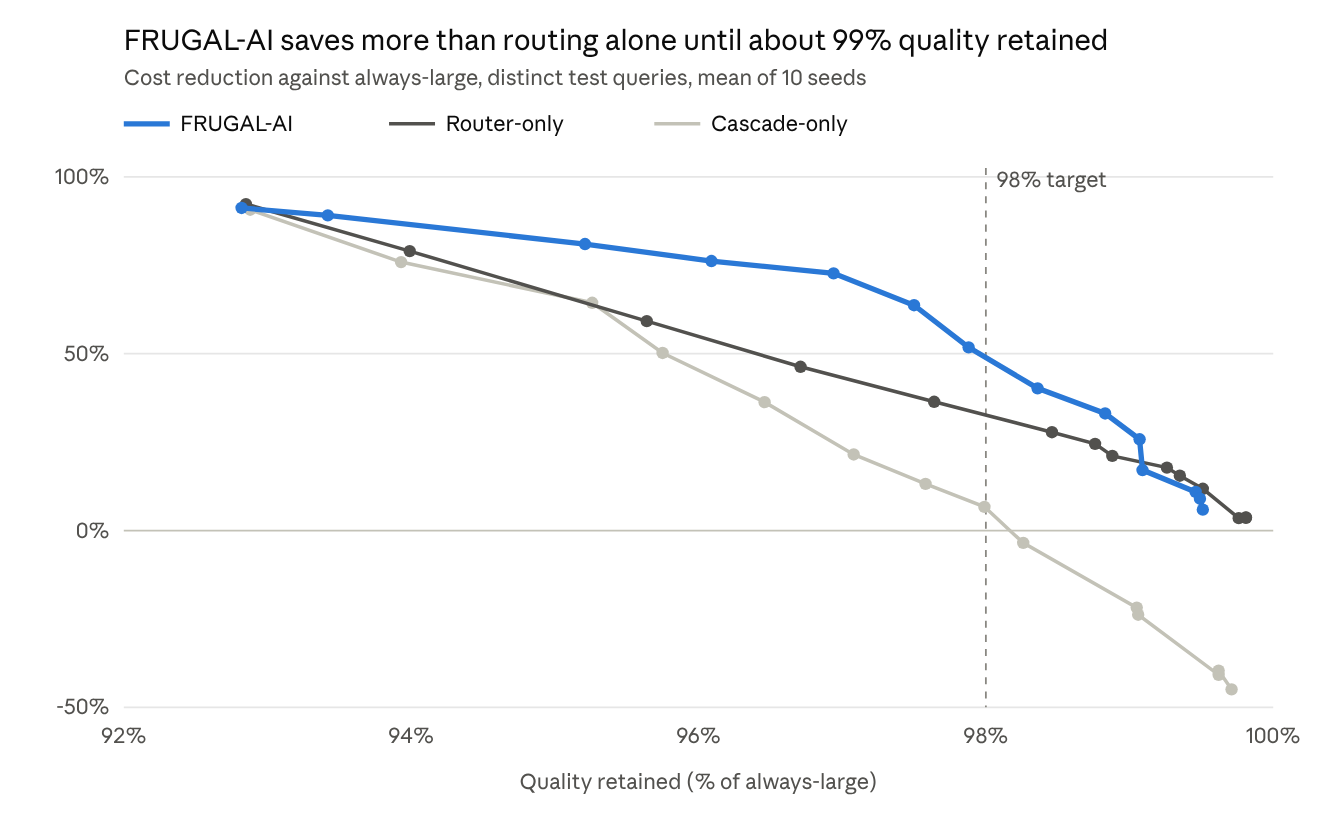
\includegraphics[width=0.92\linewidth,height=\textheight,keepaspectratio]{fig2_frontier.png}

Figure 2. Cost-quality frontier on distinct queries. Each point is one
quality tolerance, from 10\% down to 0\%. Below zero a method costs more
than always calling the large model.

Table 6. By workload at the 98\% target, distinct queries. Each cell is
cost reduction (\%) / quality retained (\%).

{\def\LTcaptype{none} % do not increment counter
\begin{longtable}[]{@{}
  >{\raggedright\arraybackslash}p{(\linewidth - 8\tabcolsep) * \real{0.1429}}
  >{\raggedright\arraybackslash}p{(\linewidth - 8\tabcolsep) * \real{0.1209}}
  >{\raggedright\arraybackslash}p{(\linewidth - 8\tabcolsep) * \real{0.1209}}
  >{\raggedright\arraybackslash}p{(\linewidth - 8\tabcolsep) * \real{0.3077}}
  >{\raggedright\arraybackslash}p{(\linewidth - 8\tabcolsep) * \real{0.3077}}@{}}
\toprule\noalign{}
\begin{minipage}[b]{\linewidth}\raggedright
Workload
\end{minipage} & \begin{minipage}[b]{\linewidth}\raggedright
Router-only
\end{minipage} & \begin{minipage}[b]{\linewidth}\raggedright
FRUGAL-AI
\end{minipage} & \begin{minipage}[b]{\linewidth}\raggedright
Router-only, per-workload floors
\end{minipage} & \begin{minipage}[b]{\linewidth}\raggedright
FRUGAL-AI, per-workload floors
\end{minipage} \\
\midrule\noalign{}
\endhead
\bottomrule\noalign{}
\endlastfoot
AIME & 90.2 / 95.8 & 64.4 / 97.6 & 26.5 / 98.0 & 71.0 / 97.1 \\
CNN/DailyMail & 5.3 / 99.5 & 34.5 / 98.1 & 23.9 / 98.1 & 19.6 / 98.9 \\
Codeforces & 1.5 / 99.9 & 14.4 / 96.6 & 11.7 / 98.6 & 8.9 / 96.6 \\
MMLU-Pro & 32.4 / 99.2 & 11.7 / 99.2 & 24.4 / 100.1 & 30.2 / 97.6 \\
MT-Bench & 31.8 / 98.1 & 78.8 / 96.1 & 26.9 / 98.8 & 25.8 / 98.3 \\
\end{longtable}
}

A target on average quality lets individual workloads fall below it:
under FRUGAL-AI, Codeforces retains 96.6\% and MT-Bench 96.1\%, and
under router-only AIME retains 95.8\%. Calibrating one setting per
workload repairs this for the router, which then meets the overall
target in every seed. It does not work for FRUGAL-AI: with 40 to 200
calibration queries per workload and many more settings to choose from,
its per-workload calibration overfits, and the overall target is met in
only 3 of 10 seeds on the replay stream.

\subsubsection{7.2 Budget adherence under drift
(RQ2)}\label{budget-adherence-under-drift-rq2}

The budget multiplier held spend under a traffic shift; the online
quality multiplier did not hold quality. When the share of easy queries
falls from 80\% to 50\%, FRUGAL-AI with fixed calibrated settings goes
from 98.8\% to 95.6\% quality retained and from 32.8\% to 21.9\% cost
reduction. Adding the online quality controller changes almost nothing:
98.7\% to 95.4\%, with 42.0\% of windows more than 1 point below the
target against 40.5\% without it. A 2\% audit rate gives about 10
quality labels per 500-request window, too few to move the multiplier in
time. The fixed cascade baseline degrades further, from 97.9\% to 93.7\%
quality retained and from a 6.7\% saving to a 12.3\% cost increase. No
method tested keeps quality at the target after the shift.

Table 7. Budget control after the shift. The budget is 15\% above the
pre-shift spend of the fixed policy.

{\def\LTcaptype{none} % do not increment counter
\begin{longtable}[]{@{}
  >{\raggedright\arraybackslash}p{(\linewidth - 6\tabcolsep) * \real{0.2308}}
  >{\raggedright\arraybackslash}p{(\linewidth - 6\tabcolsep) * \real{0.2527}}
  >{\raggedright\arraybackslash}p{(\linewidth - 6\tabcolsep) * \real{0.2088}}
  >{\raggedright\arraybackslash}p{(\linewidth - 6\tabcolsep) * \real{0.3077}}@{}}
\toprule\noalign{}
\begin{minipage}[b]{\linewidth}\raggedright
Policy
\end{minipage} & \begin{minipage}[b]{\linewidth}\raggedright
Windows over budget (\%)
\end{minipage} & \begin{minipage}[b]{\linewidth}\raggedright
Worst overshoot (\%)
\end{minipage} & \begin{minipage}[b]{\linewidth}\raggedright
Quality retained after shift (\%)
\end{minipage} \\
\midrule\noalign{}
\endhead
\bottomrule\noalign{}
\endlastfoot
Fixed thresholds & 86.0~±~21.1 & 68.5~±~27.6 & 95.6~±~1.5 \\
Online budget control & 9.0~±~10.4 & −2.0~±~5.0 & 91.5~±~2.3 \\
\end{longtable}
}

The budget multiplier keeps spend under the budget by accepting more
answers from cheaper models, which costs about 4 points of quality. It
is also conservative: because per-request cost is heavy-tailed, the
multiplier stays positive even before the shift, and spend settles well
below the budget instead of at it (Figure 3).

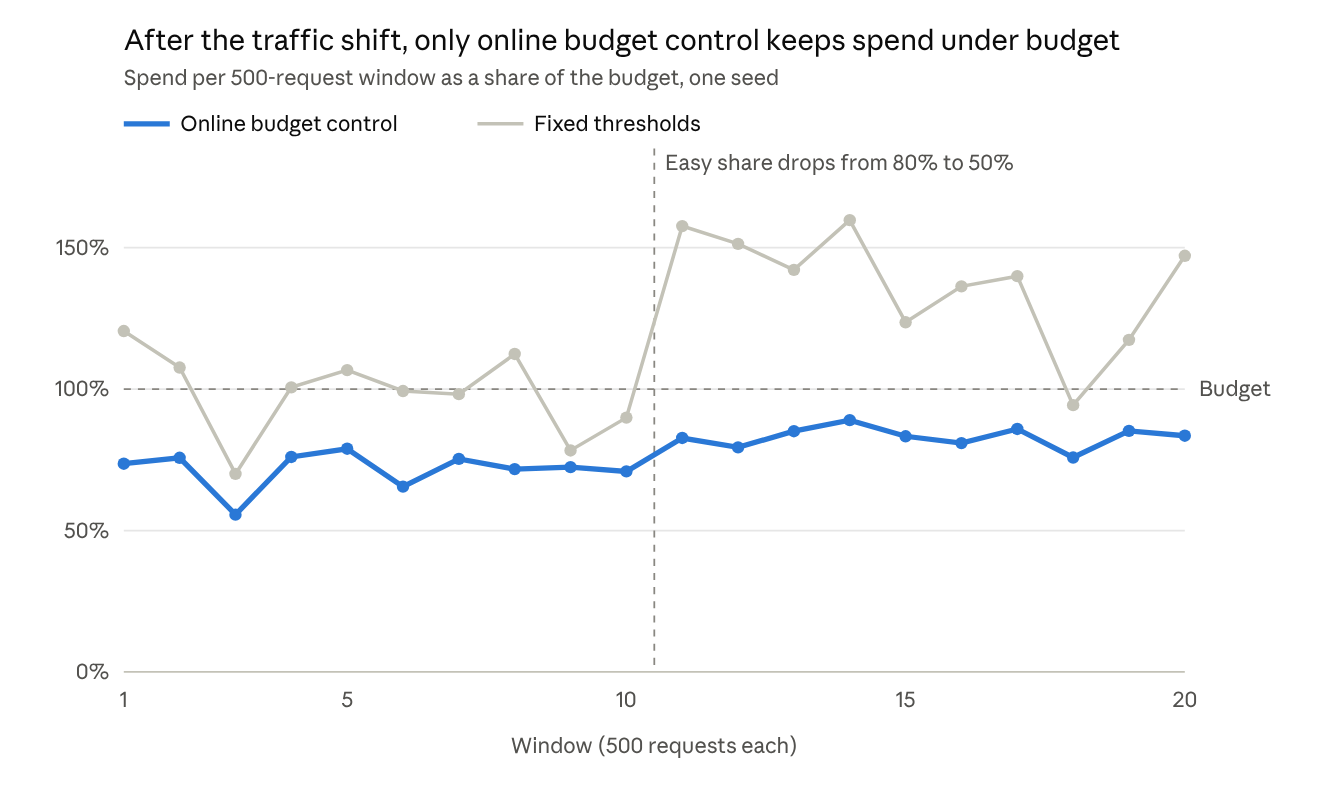
\includegraphics[width=0.92\linewidth,height=\textheight,keepaspectratio]{fig3_budget.png}

Figure 3. Spend per window for one seed. The share of easy queries drops
after window 10.

\subsubsection{7.3 Ablation (RQ3)}\label{ablation-rq3}

Table 8. Ablation on the replay stream at the 98\% target. Each variant
is recalibrated with the same rule.

{\def\LTcaptype{none} % do not increment counter
\begin{longtable}[]{@{}
  >{\raggedright\arraybackslash}p{(\linewidth - 8\tabcolsep) * \real{0.2373}}
  >{\raggedright\arraybackslash}p{(\linewidth - 8\tabcolsep) * \real{0.1525}}
  >{\raggedright\arraybackslash}p{(\linewidth - 8\tabcolsep) * \real{0.1695}}
  >{\raggedright\arraybackslash}p{(\linewidth - 8\tabcolsep) * \real{0.2034}}
  >{\raggedright\arraybackslash}p{(\linewidth - 8\tabcolsep) * \real{0.2373}}@{}}
\toprule\noalign{}
\begin{minipage}[b]{\linewidth}\raggedright
Configuration
\end{minipage} & \begin{minipage}[b]{\linewidth}\raggedright
Cost reduction (\%)
\end{minipage} & \begin{minipage}[b]{\linewidth}\raggedright
Quality retained (\%)
\end{minipage} & \begin{minipage}[b]{\linewidth}\raggedright
Seeds meeting target (\%)
\end{minipage} & \begin{minipage}[b]{\linewidth}\raggedright
Change in cost reduction (points)
\end{minipage} \\
\midrule\noalign{}
\endhead
\bottomrule\noalign{}
\endlastfoot
Full FRUGAL-AI & 50.8~±~5.2 & 98.5~±~0.7 & 70 & 0 \\
without cache & 40.4~±~8.5 & 98.7~±~0.8 & 90 & −10.4 \\
without router (cascade from smallest) & 12.8~±~7.5 & 98.5~±~0.7 & 80 &
−38.0 \\
without cascade (three-way router) & 36.0~±~8.4 & 98.6~±~0.6 & 80 &
−14.8 \\
with prompt compression & 50.8~±~5.2 & 98.5~±~0.7 & 70 & 0.0 \\
with online quality controller & 48.8~±~4.9 & 98.5~±~0.7 & 70 & −2.0 \\
\end{longtable}
}

All three core stages contribute at similar quality. The router matters
most: a cascade that always starts at the small model saves only 12.8\%.
The verifier-gated cascade adds 14.8 points on top of a three-way
router, because it lets the router start low on queries it is unsure
about and still recover. The cache adds 10.4 points on this stream, less
than its 28\% hit rate, since many repeated requests would have been
served cheaply anyway. Allowing prompt compression changes nothing,
because the calibration never selects it. The online quality controller
costs 2 points, the price of its audit calls, and returns no quality.

\subsubsection{7.4 Sensitivity and
overhead}\label{sensitivity-and-overhead}

Results move mainly with the share of repeated requests and the cache
threshold.

Table 9. Sensitivity of FRUGAL-AI on the replay stream, 98\% target.

{\def\LTcaptype{none} % do not increment counter
\begin{longtable}[]{@{}
  >{\raggedright\arraybackslash}p{(\linewidth - 8\tabcolsep) * \real{0.2745}}
  >{\raggedright\arraybackslash}p{(\linewidth - 8\tabcolsep) * \real{0.1765}}
  >{\raggedright\arraybackslash}p{(\linewidth - 8\tabcolsep) * \real{0.1961}}
  >{\raggedright\arraybackslash}p{(\linewidth - 8\tabcolsep) * \real{0.1765}}
  >{\raggedright\arraybackslash}p{(\linewidth - 8\tabcolsep) * \real{0.1765}}@{}}
\toprule\noalign{}
\begin{minipage}[b]{\linewidth}\raggedright
Setting
\end{minipage} & \begin{minipage}[b]{\linewidth}\raggedright
Cost reduction (\%)
\end{minipage} & \begin{minipage}[b]{\linewidth}\raggedright
Quality retained (\%)
\end{minipage} & \begin{minipage}[b]{\linewidth}\raggedright
Cache hit rate (\%)
\end{minipage} & \begin{minipage}[b]{\linewidth}\raggedright
False-hit rate (\%)
\end{minipage} \\
\midrule\noalign{}
\endhead
\bottomrule\noalign{}
\endlastfoot
\(\tau_{\mathrm{cache}}\) = 0.80 & 52.6~±~4.9 & 97.6~±~0.9 & 30.9 &
1.53 \\
\(\tau_{\mathrm{cache}}\) = 0.85 & 51.3~±~5.2 & 98.5~±~0.9 & 29.8 &
0.62 \\
\(\tau_{\mathrm{cache}}\) = 0.90 & 50.6~±~5.4 & 98.7~±~0.9 & 28.5 &
0.36 \\
\(\tau_{\mathrm{cache}}\) = 0.95 & 50.1~±~5.4 & 99.0~±~0.8 & 26.8 &
0.16 \\
Repeat share 0\% & 33.4~±~7.2 & 98.2~±~0.5 & 0.7 & 0.70 \\
Repeat share 15\% & 43.2~±~6.5 & 98.3~±~0.6 & 14.4 & 0.67 \\
Repeat share 30\% & 53.6~±~6.7 & 98.5~±~0.6 & 28.3 & 0.63 \\
Repeat share 50\% & 66.9~±~5.9 & 98.6~±~0.5 & 47.7 & 0.45 \\
Online quality controller, ρ = 0.5\% & 51.5~±~6.1 & 98.5~±~0.7 & 28.5 &
0.60 \\
Online quality controller, ρ = 2\% & 48.8~±~4.9 & 98.5~±~0.7 & 28.5 &
0.60 \\
Online quality controller, ρ = 5\% & 46.8~±~4.8 & 98.5~±~0.7 & 28.5 &
0.60 \\
Online quality controller, η = 0.5 & 52.6~±~8.5 & 97.6~±~1.3 & 28.5 &
0.60 \\
\end{longtable}
}

A wrong cache hit almost always returns a wrong answer, so quality
tracks the false-hit rate closely: moving \(\tau_{\mathrm{cache}}\) from
0.80 to 0.95 raises quality retained from 97.6\% to 99.0\% for 2.5
points of saving. The saving grows from 33.4\% with no repeats to 66.9\%
when half the requests are repeats. With the online quality controller,
a higher audit rate only adds cost. The calibrated values were
\(\tau_{\mathrm{cache}}\) = 0.89, α = 0.055 and λ = 23.2 on average,
giving acceptance thresholds of 0.66 for the small model and 0.45 for
the mid model. Overhead per request is 4.4 ms for the embedding and
under 0.01 ms for the routing decision; a verifier call takes 3.7 s on
average.

\subsection{8. Discussion, Limitations and
Ethics}\label{discussion-limitations-and-ethics}

FRUGAL-AI's savings depend on how much quality the operator is willing
to trade and on how repetitive the traffic is; at the strictest targets
a plain router is as good and easier to calibrate.

When it helps most. The combined pipeline pays off when a loss of 1.5 to
3 points of quality is acceptable, when traffic has many repeats, and
when latency is not critical, since the verifier adds seconds to the
slowest requests. When the target is within 1 point of the strongest
model, or when each task type must meet the target on its own, a
calibrated router is the safer choice. Three practical lessons follow.
Tune against a margin, not the bare target, and report how often the
target is met. Give the cache an explicit share of the error budget. Do
not expect a small audit sample to steer quality online; recalibrate
offline when traffic shifts.

\textbf{Limitations.}

\begin{itemize}
\tightlist
\item
  \textbf{Router training cost:} labelling requires running every pool
  model on a training set once. This one-time cost should be reported
  and amortized over expected traffic.
\item
  \textbf{Quality measurement:} LLM judges can be biased toward longer
  answers or their own model family. We use task metrics where possible;
  we did not collect human ratings.
\item
  \textbf{Cache risks:} wrong reuse of an answer to a similar but
  different question can harm users. Time-to-live, context hashing and a
  calibrated threshold reduce but do not remove this risk.
\item
  \textbf{Model churn:} prices and models change often, so the router
  needs retraining. Recalibration needs fresh outputs from every pool
  model.
\item
  \textbf{Theory assumptions:} we give no formal guarantee. The
  calibration margin is a heuristic, and the online-control results we
  cite assume i.i.d. requests and exact feedback.
\end{itemize}

Limitations of this evaluation.

\begin{itemize}
\tightlist
\item
  Target not always met: with the margin, FRUGAL-AI meets the 98\%
  target in 7 of 10 seeds on the replay stream and in 5 of 10 on
  distinct queries. The margin makes meeting the target likely, not
  certain.
\item
  Tuning rule chosen after a first evaluation: see the disclosure in
  Section 6.5. A fresh test set would be needed to rule out any benefit
  from that choice.
\item
  Single model family: all three models are Claude models, and the large
  model also judges the summaries and dialogues, including its own.
\item
  Seeds are not independent model samples: each query was answered once
  per model, and seeds redraw only the split, the stream and the audits.
\item
  Small test sets: about 440 queries per split, and 40 to 200 per
  workload.
\item
  Synthetic traffic: the 30\% repeat share and the drift scenario are
  assumptions, not measurements of real traffic.
\item
  Baselines: the 2026 systems named in Section 2 (ParetoBandit,
  WISERouter, Cascade Routing, Conformal Cascade) were not implemented.
\item
  Cost method: costs are tokens times list prices from command-line
  calls with a measured overhead subtracted, not metered API bills.
\item
  Possible contamination: the Codeforces problems date from 2021 and
  earlier, so the models may have seen them in training.
\end{itemize}

\textbf{Ethics and fairness.} Routing by predicted difficulty could give
some user groups, languages or dialects systematically weaker models. We
recommend reporting quality per language or user segment and adding
per-segment quality constraints where needed. Cache entries must not
leak one user's private data to another, so caches should be partitioned
by tenant and exclude personal data.

\textbf{Environmental impact.} Fewer calls to large models also cut
energy use. Reporting estimated kWh alongside cost supports Green AI
reporting practice {[}18{]}.

\subsection{9. Conclusion and Future
Work}\label{conclusion-and-future-work}

Calibrating a semantic cache, a difficulty router and a verifier-gated
cascade together, against one quality target with a margin, cut LLM
inference cost by 50.8\% at 98.5\% of the strongest model's quality on a
stream with 30\% repeated requests. That is about twice the saving of
routing or caching alone, and the advantage over routing holds at
matched quality up to 98.5\% quality retained. At a 99\% target the
combined pipeline is no better than a router. Prompt compression, an
audit-driven online quality controller and per-workload floors for the
full pipeline did not pay off, while an online budget multiplier held
spend under a traffic shift at a measurable cost in quality.

Future work includes four directions:

\begin{itemize}
\tightlist
\item
  Contextual-bandit routers that learn from live feedback without full
  offline labelling.
\item
  Joint routing over models and decoding settings, such as quantized
  variants and speculative decoding.
\item
  Per-segment fairness constraints built into the controller.
\item
  Extension to multi-step agent workflows, where one task triggers many
  model and tool calls.
\end{itemize}

\subsection{Declarations}\label{declarations}

Funding. This research received no external funding. All model usage was
paid for by the author.

Conflict of interest. The author declares no conflict of interest. The
author is an independent researcher with no affiliation to, or support
from, the provider of the models evaluated.

Use of AI tools. The author used Claude (Anthropic), through Claude
Code, to draft the manuscript text, to write the experiment and analysis
code, and to produce the tables and figures from the logged results. The
models evaluated in the experiments are also Claude models. The author
directed the work, reviewed and edited the output, checked the results
against the released code and logs, and takes full responsibility for
the content of this paper.

\subsection{Code and Data
Availability}\label{code-and-data-availability}

The code, the logged model outputs and the results are available at
\url{https://github.com/vijayakumargr/frugal-ai}. The repository
rebuilds the query set from the public benchmarks and reproduces every
table in this paper without model calls. It also contains the first
evaluation described in Section 6.5. Version 1.0.0 is archived on
Zenodo, https://doi.org/10.5281/zenodo.24202801.

\subsection{References}\label{references}

Authors, titles, venues and years were checked on 13 November 2026
against arXiv, Crossref and the proceedings pages. Three entries were
corrected: the title and venue of {[}3{]} and the author lists of
{[}4{]} and {[}7{]}. Entries {[}30{]} to {[}36{]} are preprints and may
have been published since; check them again, and format the list to the
journal's style, before submission.

\begin{enumerate}
\def\labelenumi{\arabic{enumi}.}
\tightlist
\item
  L. Chen, M. Zaharia and J. Zou, ``FrugalGPT: How to use large language
  models while reducing cost and improving performance,''
  arXiv:2305.05176, 2023.
\item
  D. Ding et al., ``Hybrid LLM: Cost-efficient and quality-aware query
  routing,'' in Proc. ICLR, 2024.
\item
  I. Ong et al., ``RouteLLM: Learning to route LLMs from preference
  data,'' in Proc. ICLR, 2025.
\item
  P. Aggarwal, A. Madaan et al., ``AutoMix: Automatically mixing
  language models,'' in Proc. NeurIPS, 2024.
\item
  F. Bang, ``GPTCache: An open-source semantic cache for LLM
  applications enabling faster answers and cost savings,'' in Proc. 3rd
  Workshop for Natural Language Processing Open Source Software
  (NLP-OSS), 2023, pp.~212--218.
\item
  W. Kwon et al., ``Efficient memory management for large language model
  serving with PagedAttention,'' in Proc. SOSP, 2023.
\item
  Y. Li, B. Dong, C. Lin and F. Guerin, ``Compressing context to enhance
  inference efficiency of large language models,'' in Proc. EMNLP, 2023.
\item
  H. Jiang, Q. Wu, C.-Y. Lin, Y. Yang and L. Qiu, ``LLMLingua:
  Compressing prompts for accelerated inference of large language
  models,'' in Proc. EMNLP, 2023.
\item
  H. Jiang et al., ``LongLLMLingua: Accelerating and enhancing LLMs in
  long context scenarios via prompt compression,'' in Proc. ACL, 2024.
\item
  G. Hinton, O. Vinyals and J. Dean, ``Distilling the knowledge in a
  neural network,'' arXiv:1503.02531, 2015.
\item
  E. Frantar, S. Ashkboos, T. Hoefler and D. Alistarh, ``GPTQ: Accurate
  post-training quantization for generative pre-trained transformers,''
  in Proc. ICLR, 2023.
\item
  J. Lin et al., ``AWQ: Activation-aware weight quantization for LLM
  compression and acceleration,'' in Proc. MLSys, 2024.
\item
  Y. Leviathan, M. Kalman and Y. Matias, ``Fast inference from
  transformers via speculative decoding,'' in Proc. ICML, 2023.
\item
  A. Badanidiyuru, R. Kleinberg and A. Slivkins, ``Bandits with
  knapsacks,'' in Proc. IEEE FOCS, 2013, pp.~207--216.
\item
  M. Mahdavi, R. Jin and T. Yang, ``Trading regret for efficiency:
  Online convex optimization with long term constraints,'' JMLR,
  vol.~13, 2012.
\item
  H. Yu, M. J. Neely and X. Wei, ``Online convex optimization with
  stochastic constraints,'' in Proc. NIPS, 2017.
\item
  E. Strubell, A. Ganesh and A. McCallum, ``Energy and policy
  considerations for deep learning in NLP,'' in Proc. ACL, 2019,
  pp.~3645--3650.
\item
  R. Schwartz, J. Dodge, N. A. Smith and O. Etzioni, ``Green AI,''
  Commun. ACM, vol.~63, no. 12, pp.~54--63, 2020.
\item
  C. Guo, G. Pleiss, Y. Sun and K. Q. Weinberger, ``On calibration of
  modern neural networks,'' in Proc. ICML, 2017.
\item
  A. N. Angelopoulos and S. Bates, ``A gentle introduction to conformal
  prediction and distribution-free uncertainty quantification,''
  arXiv:2107.07511, 2021.
\item
  D. Hendrycks et al., ``Measuring massive multitask language
  understanding,'' in Proc. ICLR, 2021.
\item
  K. Cobbe et al., ``Training verifiers to solve math word problems,''
  arXiv:2110.14168, 2021.
\item
  M. Chen et al., ``Evaluating large language models trained on code,''
  arXiv:2107.03374, 2021.
\item
  A. See, P. J. Liu and C. D. Manning, ``Get to the point: Summarization
  with pointer-generator networks,'' in Proc. ACL, 2017, pp.~1073--1083.
\item
  L. Zheng et al., ``Judging LLM-as-a-judge with MT-Bench and Chatbot
  Arena,'' in Proc. NeurIPS Datasets and Benchmarks Track, 2023.
\item
  A. N. Angelopoulos, S. Bates, A. Fisch, L. Lei and T. Schuster,
  ``Conformal risk control,'' in Proc. ICLR, 2024.
\item
  Y. Wang et al., ``MMLU-Pro: A more robust and challenging multi-task
  language understanding benchmark,'' in Proc. NeurIPS Datasets and
  Benchmarks Track, 2024.
\item
  Y. Li et al., ``Competition-level code generation with AlphaCode,''
  Science, vol.~378, no. 6624, pp.~1092--1097, 2022.
\item
  AI-MO, ``aimo-validation-aime,'' dataset of 90 AIME problems from 2022
  to 2024, Hugging Face,
  https://huggingface.co/datasets/AI-MO/aimo-validation-aime.
\item
  A. Taberner-Miller, ``ParetoBandit: Budget-paced adaptive routing for
  non-stationary LLM serving,'' arXiv:2604.00136, 2026.
\item
  Y. Li, Z. Gao and L. V. S. Lakshmanan, ``WISERouter: LLM routing with
  workload budget constraint,'' arXiv:2607.23765, 2026.
\item
  D. Sheshanarayana, R. S. Pal, M. Sinha and T. Dasgupta, ``GAR:
  Carbon-aware routing for LLM inference via constrained optimization,''
  arXiv:2605.11603, 2026.
\item
  P. Panda, R. Magazine, C. Devaguptapu, S. Takemori and V. Sharma,
  ``Adaptive LLM routing under budget constraints,'' in Findings of
  EMNLP, 2025.
\item
  J. Dekoninck, M. Baader and M. Vechev, ``A unified approach to routing
  and cascading for LLMs,'' arXiv:2410.10347, 2024.
\item
  Y. Dou, S. Lian and S. Li, ``Conformal Cascade: Distribution-free
  accuracy guarantees for multi-tier LLM inference,'' arXiv:2607.25018,
  2026.
\item
  A. Valkanas, S. Pal, P. Rumiantsev, Y. Zhang and M. Coates, ``C3PO:
  Optimized large language model cascades with probabilistic cost
  constraints for reasoning,'' arXiv:2511.07396, 2025.
\item
  Y. Moslem and J. D. Kelleher, ``Dynamic model routing and cascading
  for efficient LLM inference: A survey,'' Transactions on Machine
  Learning Research, 2026.
\end{enumerate}

\end{document}
